\begin{center}
\section{Determinazione dell'\textit{energy gap} del semiconduttore}
\medskip
\end{center}
{\color{gray}\hrule}
\medskip
Nota la relazione $(\lambda \circ \#_{ch} )(x)$, che permette di legare le unità arbitrarie alla lunghezza d'onda, si può procedere con lo studio della fotocorrente e della trasmittanza per la stima dell'\textit{energy gap} del Seleniuro di Gallio, proporzionali rispettivamente all'intensità luminosa assorbita e a quella trasmessa dal campione.\\ Da una prima analisi qualitativa si ottiene che il colore trasmesso dal semiconduttore posto in controluce è nel range del rosso: è quindi possibile dedurre che il campione si comporta come un buon conduttore \textit{ottico} nel range  [620nm - 700nm] e predire che l'\textit{energy gap} sia un valore compreso tra 1.8eV e 2eV.


\subsection{Spettro di emissione della lampada alogena}
Si acquisisce ora lo spettro di riferimento della radiazione emessa dalla lampada alogena in assenza del campione di SeGa: come atteso per un corpo nero, le misure della tensione ai capi del fotodiodo $V_{0,f}$ in funzione della lunghezza d’onda selezionata dal monocromatore $\lambda$ danno un'indicazione della non uniformità della sorgente luminosa, suggerendo di normalizzare successivamente i dati di trasmittanza e fotocorrente.  \\
%A tal fine si sono acquisite ?? misure delle distanze picco-picco $V_{pp,f}$ in funzione della lunghezza d'onda, impostata di volta in volta ruotando unidirezionalmente la vite micrometrica  del monocromatore. \\ questa parte non mi sembra serva

%nota per Sofi: ho fatto picco a picco, l'ho anche scritto nel grafico, non penso serva specificarlo, se scrivo pp significa per forza due volte V. io non ho fatto nessun fit di corpo nero, non l'ho visto nella scheda.$
\begin{figure}[H]
    \centering
    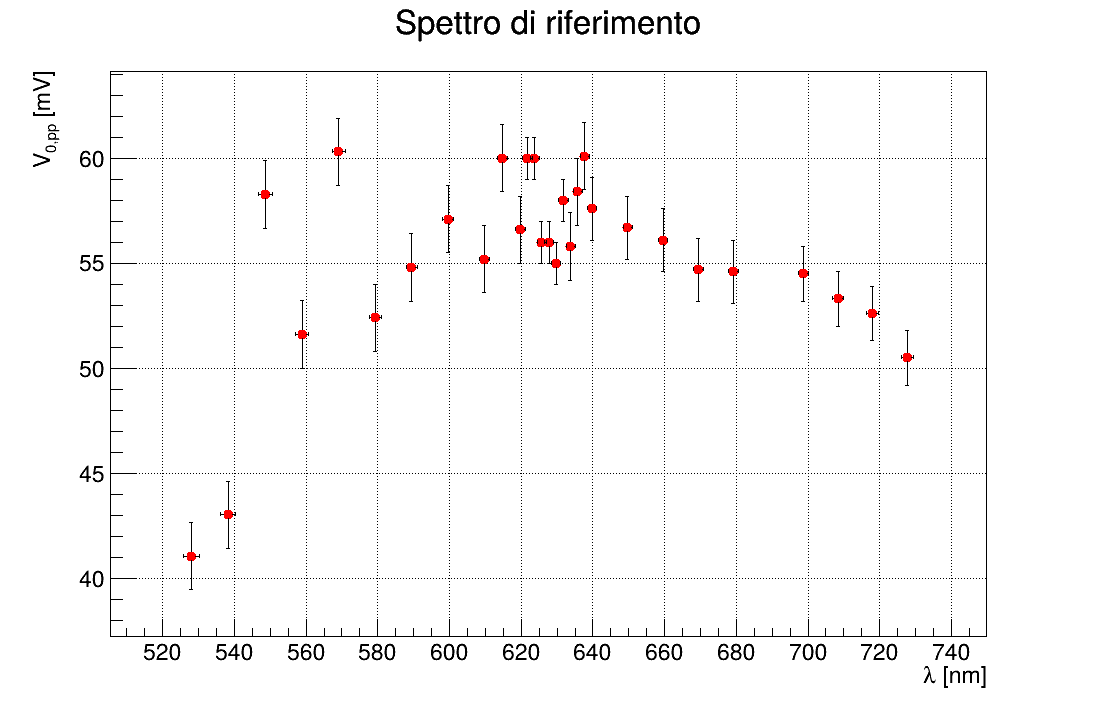
\includegraphics[width=0.85\linewidth]{riferimento.png}
    \caption{ \footnotesize Spettro di riferimento, a meno di costanti moltiplicative, dell'intensità luminosa della radiazione emessa dalla lampada alogena, misurata come intensità assorbita dal fotodiodo ($\lambda_i$,$V_{0,f,pp}$).}
    \label{fig:fondo}
\end{figure}
Dal grafico \ref{fig:fondo} si osserva in particolare che l'intensità luminosa diminuisce significativamente in corrispondenza delle lunghezze d'onda del violetto. Inoltre, i dati non mostrano un andamento continuo, le misure che si discostano notevolmente dalle altre sono molto probabilmente compromesse dalla radiazione ambientale. 
\newpage
\textit{Osservazione.} La misura di $V_{0,pp}$, proporzionale all'intensità luminosa assorbita dal fotodiodo, è in questo caso la miglior approssimazione dell'intensità luminosa incidente sul campione ottenuta dal sistema di misura, in quanto si dovrebbe anche tenere conto delle riflettività e dell'efficienze relative del campione e del fotodiodo. Tuttavia, ai fini dell'esperienza interessano soltanto i rapporti in altezza tra le misure e non le altezze.

\subsection{Determinazione dell'\textit{energy gap} $E_{g,SeGa}$.}
Dopo aver allineato lungo l'asse ottico il campione, si osserva che l'intensità della radiazione trasmessa - cioè quella incidente sul fotodiodo - decresce rapidamente fino ad annullarsi per lunghezze d’onda inferiori a circa $640$nm, confermando l'ipotesi iniziale; il punto di massima pendenza identifica dunque la soglia di assorbimento $\lambda_g$ del materiale di cui è composto il semiconduttore.
% Infatti, per lunghezze d’onda inferiori a $\lambda_g$ - dunque per energie maggiori - i fotoni incidenti hanno abbastanza energia per promuovere elettroni dalla banda di valenza alla banda di conduzione, causando l'assorbimento di tale radiazione. \\ Infine, dalla relazione tra energia del fotone e lunghezza d’onda $\lambda_g$ è possibile ricavare una stima dell’\textit{energy gap} del materiale $E_{g,SeGa}$:
%\begin{equation}
  %  E=\frac{hc}{\lambda_g}
   % \label{eq:energy}
%\end{equation}

\begin{figure}[H]
    \centering
    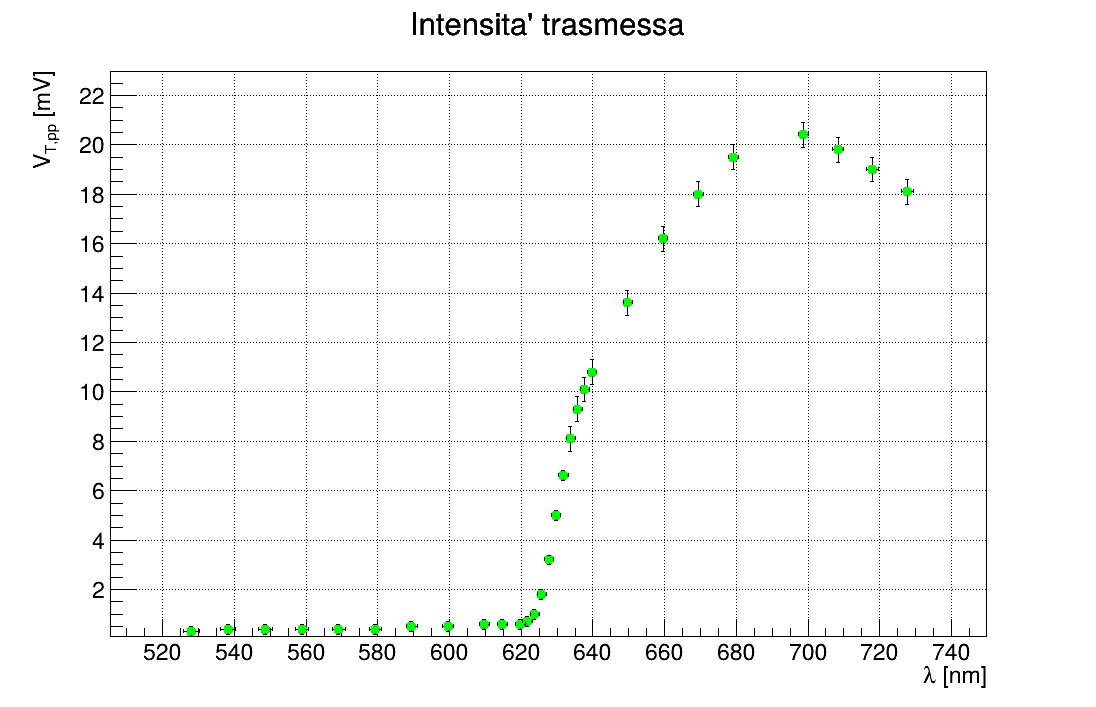
\includegraphics[width=0.85\linewidth]{trasmessa.png}
    
    \caption{\footnotesize Coppie di valori ($\lambda$,$V_{f,pp}$), con $V_{f,pp}$ direttamente proporzionale all'intensità trasmessa dal campione.}
    \label{fig:enter-label}
\end{figure}

\subsubsection{Trasmittanza ottica e fotocorrente}
Per poter studiare l'andamento della trasmittanza e della fotocorrente in funzione della lunghezza d'onda, si fa variare quest'ultima ruotando la vite micrometrica del monocromatore a passi di 10 u.a., intensificando le misure quando si osserva sull'oscilloscopio un cambiamento brusco dell'andamento delle cadute di potenziale $V_{f}$ e $V_{c}$ ai capi delle rispettive resistenze di carico, $R_f$ e $R_c$.

La trasmittanza è definita operativamente dal rapporto tra l'intensità trasmessa dal campione e quella incidente, a meno di fattori moltiplicativi risulta essere: $$T=\frac{V_{f,pp}}{V_{0,f,pp}}$$ \\
Invece, la fotocorrente, generata dalla radiazione elettromagnetica incidente in seguito alla creazione di coppie elettrone-lacuna, è esprimibile dalla legge di Ohm macroscopica come $$i_{ph}=\frac{V_{c}}{R_c}$$ con $R_c= (1.00 \pm 0.05)M\Omega$. 
%devo specificare che la corrente è picco a picco? io non so se è stata divisa per 2

Mentre la trasmittanza risulta già normalizzata per definizione, la fotocorrente $i_{ph}$ va normalizzata per ciascun valore di $\lambda$ tramite la relazione $$i_{n}=\frac{i_{ph}}{V_{0}}$$ Le coppie di valori ($\lambda_j$,$T_j$) e ($\lambda_j$,$i_{n,j}$) ottenute sono riportate rispettivamente nelle tabelle \ref{tab:trasmittanza} e \ref{tab:fotocorrente} in appendice. Si graficano tali valori e, individuato un intervallo spettrale opportuno, si interpolano entrambe le coppie con la curva sigmoide \ref{eq:sigmoide}\ per ricavare il punto di flesso, e di conseguenza la corrispondente $\lambda_g$ del semiconduttore. \\
\begin{equation}
    S(\lambda) = b + \frac{A}{1+e^ {\pm \frac{\lambda-\lambda_g}{\Delta \lambda}}}
    \label{eq:sigmoide}
\end{equation}
dove $\lambda_g$ e $\Delta\lambda$ rappresentano rispettivamente la lunghezza d'onda di soglia del semiconduttore e la sua incertezza; il segno $\pm$ è, rispettivamente, relativo alla fotocorrente e alla trasmittanza.
\begin{figure}[H]
    \centering
    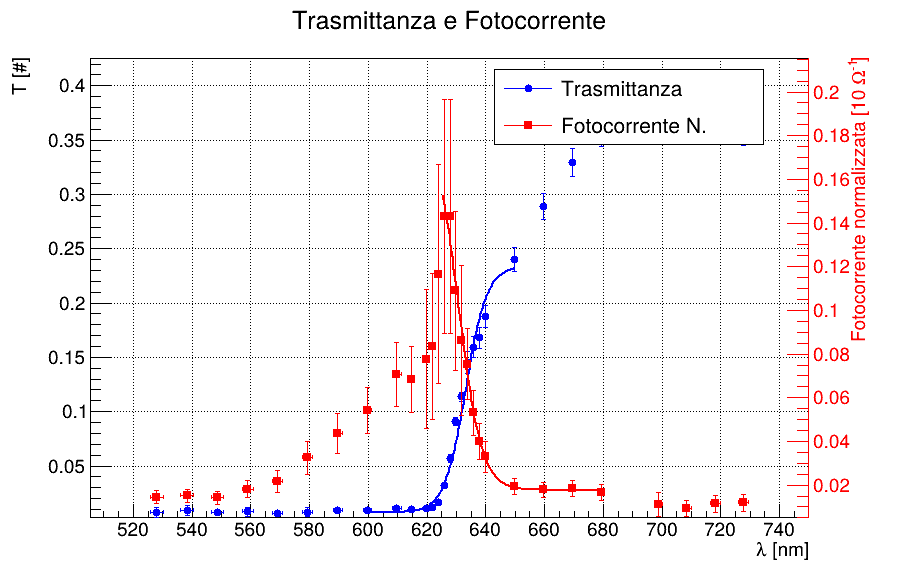
\includegraphics[width=0.85\linewidth]{trasmittanza.png}
    \caption{\footnotesize Coppie di valori ($\lambda_i$,$T_i$) e ($\lambda_i$,$i_{n,i}$) con i rispettivi fit.}
    \label{fig:enter-label}
\end{figure}
\newpage
\begin{table}[H]
\centering
\begin{tabular}{|c|c|c|}
\hline 
                  & \textbf{Fotocorrente} & \textbf{Trasmittanza} \\ \hline

$b$               &   $(0.018 \pm 0.002) 10 \Omega^{-1}$  & $(0.234 \pm 0.012) $           \\
$A$               &   $(0.17 \pm 0.13) 10 \Omega^{-1}$ & $ (-0.227\pm 0.013) $ \\
$\lambda_g$       &   $(631 \pm 7)$nm & $ (633.1 \pm 0.7)$nm \\ 
$\Delta\lambda$   &   $(4 \pm 2)$nm & $ (3.6 \pm 0.4) $nm\\ 
$\chi ^2$         &   $0.3$            & $9$          \\ 
d.o.f             &   $8$            & $10$          \\ 
\hline
\end{tabular}
\caption{Risultati dei fit.}
\label{tab:fotocorrente}
\end{table}

\textit{Osservazione.} Il $\chi ^2$ del fit per la fotocorrente risulta molto piccolo, ciò si può in parte attribuire al peso che l'errore sulla resistenza ha avuto nella stima dell'errore sulla fotocorrente.




\subsubsection{Misura sperimentale di $E_{g,SeGa}$}
Da ciascun fit si ricava una stima dell'\textit{energy gap} $E_{g,SeGa}$ tramite la formula $ E=\frac{hc}{\lambda_g} $
$$ E_T = (1.959 \pm0.011) \text{eV} $$ 
$$ E_I = (1.966 \pm 0.012)\text{eV}$$  
Dopo aver verificato la compatabilità statistica tra le due stime, si fa una media pesata  di queste ricavandone una stima finale dell'\textit{energy gap}:
$$E_g= (1.962 \pm 0.008)\text{eV}$$  
